\section{Formal proofs of hard problems}\label{sec:cases}

Several of the hardest problems of mathematics now have proofs that a machine has checked line by line, and four of these formal proofs were written with the help of artificial intelligence \cite{Ant26,ZDC26,HBL26,OAI26}. They are the natural test of the theory: each is a long chain of steps, each step has a check, and each records which steps were hard. This section reads six of them in the language of Sections~\ref{sec:chains} and~\ref{sec:agents}, states what a BLLM adds and what it does not, and describes the package that implements the system.

\subsection{Six problems}

\begin{figure*}[t]
\centering
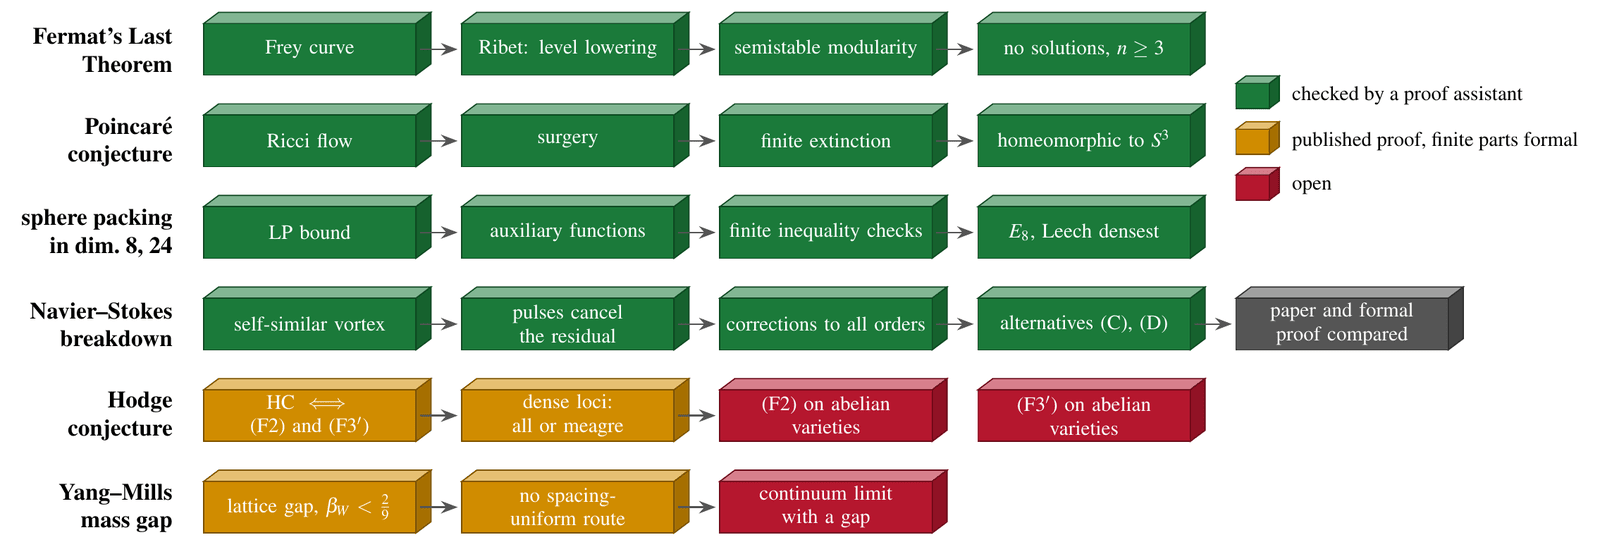
\includegraphics[width=0.98\textwidth]{figures/fig_cases}
\caption{The main steps of the six proofs of Table~\ref{tab:cases}. Green steps are checked by a proof assistant, gold steps have published proofs whose formal checks cover only finite parts, red steps are open, and grey marks the comparison of the Navier--Stokes paper with its formal proof \cite{BCH26}. The two Hodge statements (F2) and (F3$'$) are independent, and both are needed.}
\label{fig:cases}
\end{figure*}

Table~\ref{tab:cases} and Fig.~\ref{fig:cases} list the problems, the formal results and the steps that remain. Four are settled: Fermat's Last Theorem by Wiles and by Taylor and Wiles \cite{Wil95,TW95}, formalised in Lean~4 in September 2026 by dozens of Claude agents in eleven days on the Prove2Me platform, along the simplified proof of Darmon, Diamond and Taylor, in about thirteen million lines with $29{,}500$ theorems in the final proof and only the three standard axioms \cite{Ant26,CML26,DDT95}; the Poincar\'e conjecture by Perelman, now formalised in Lean~4 with Mathlib following the account of Morgan and Tian \cite{ZDC26}; the sphere packing problem in dimensions $8$ and $24$ \cite{Via17,CKM17}, formalised by Hariharan, Birkbeck, Lee, Ma, Mehta, Poiroux and Viazovska and completed by Math, Inc. \cite{HBL26}; and finite-time breakdown of the three-dimensional Navier--Stokes equations with forcing, alternatives (C) and (D) of the official description of the Millennium problem, proved by OpenAI for every positive viscosity in a paper of 165 pages and in Lean \cite{OAI26}. Each formal development is archived with a record of an independent build \cite{ArcNS,ArcPC,ArcSP}. Two are open: the Hodge conjecture, which the first two authors reduced to two statements (F2) and (F3$'$) about abelian varieties \cite{BB26c}, and the existence of Yang--Mills theory with a mass gap, for which they proved a lattice mass gap for four-dimensional $\mathrm{SU}(2)$ up to the coupling $\beta_{W}=\frac29$, the limit of single-link Dobrushin arguments \cite{BB26d}.\footnote{D.~Bhattacharjee and U.~Bhattacharya, \emph{Dense algebraic loci of Hodge classes}, Hexagon preprint hexagon:2610.00315v1 (17 October 2026), with Lean~4 archive doi:10.5281/zenodo.23439578 \cite{BB26c}. The paper proves that the Hodge conjecture is equivalent to two statements about abelian varieties, that the locus on which either holds is dense in every family and is either the whole family or a meagre set, builds for each statement the object it needs next and proves at which step it stops. The second work, \emph{Lattice Yang--Mills theory: spacing-uniform obstructions, the mass gap up to the Dobrushin ceiling, and Lean certificate}, Zenodo (2026), doi:10.5281/zenodo.23449466 \cite{BB26d}, also proves that lattice inequalities uniform in the spacing cannot produce the continuum mass gap, and isolates the remaining step as one hypothesis on the ratio of the lattice gap to the spacing.}

\begin{table*}[t]
\caption{Six problems with machine-checked or published proofs, in the language of the moves of Section~\ref{ssec:moves}. ``Formal'' names the proof checker of the archived development; the last column names the moves on which the proof rests.}
\label{tab:cases}
\centering
\footnotesize
\setlength{\tabcolsep}{4pt}
\begin{tabular}{@{}p{0.13\textwidth}p{0.29\textwidth}p{0.08\textwidth}p{0.24\textwidth}p{0.17\textwidth}@{}}
\toprule
Problem & What is proved & Formal & What remains & Moves \\
\midrule
\rr Fermat's Last Theorem & \rr modularity of semistable elliptic curves, hence the theorem \cite{Wil95,TW95,Ant26} & Lean~4 & \rr nothing & \rr bypass (Frey, Ribet), residual (Taylor--Wiles) \\
\rr Poincar\'e conjecture & \rr Hamilton--Perelman Ricci flow with surgery \cite{ZDC26} & Lean~4 & \rr nothing & \rr construction, residual (surgery) \\
\rr Sphere packing in dimensions 8, 24 & \rr $E_{8}$ and the Leech lattice are densest \cite{Via17,CKM17,HBL26} & Lean~4 & \rr nothing in dimensions 8, 24 & \rr construction, trivialization \\
\rr Navier--Stokes breakdown & \rr alternatives (C), (D) for every viscosity \cite{OAI26} & Lean~4 & \rr the correspondence of paper and formal proof \cite{BCH26} & \rr construction, residual, blow-up \\
\rr Hodge conjecture & \rr equivalence with (F2) and (F3$'$); dense loci \cite{BB26c} & \rr Lean~4, finite parts & \rr (F2), (F3$'$) & \rr bypass, strong then weak \\
\rr Yang--Mills mass gap & \rr lattice gap for $\beta_{W}<\frac29$; no spacing-uniform route \cite{BB26d} & \rr Lean~4, finite parts & \rr continuum limit with a gap & \rr construction, strong then weak, residual \\
\bottomrule
\end{tabular}
\end{table*}

The history of the problems contains the moves of Section~\ref{ssec:moves}. Wiles announced a proof in 1993 in which one step failed; the repair with Taylor replaced it by a different argument \cite{TW95}, a residual move on a single step of a long chain. The Navier--Stokes construction of \cite{OAI26} builds a self-similar vortex, cancels the singular part of its momentum residual by oscillatory pulses and corrects what is left to every order: construction, residual and blow-up in one argument. The sphere packing proofs reduce optimality to the existence of auxiliary functions whose inequalities are checked by finite computations, a trivialization. The Hodge reduction replaces the conjecture by statements on abelian varieties through known theorems, a bypass, and weakens one of them to (F3$'$), a step down the ladder of strong then weak.

\subsection{What a BLLM adds, and what it does not}

Three of the theorems of this paper speak directly to these proofs.

First, Theorem~\ref{thm:gating}. A formal development checks every step of the formal argument, not the steps of the paper it formalises. Bastounis, Circelli and Hansen argue that the Lean proof of \cite{OAI26} does not follow the argument of the paper, and that a faithful translation of a natural-language proof is not computable in general \cite{BCH26}. Whatever the outcome of that discussion, a natural-language argument whose only certificate is a formal proof of its final statement is checked at its outcome, and Theorem~\ref{thm:gating} shows that certification at the outcome is exponentially more expensive in the number of steps than certification step by step. A BLLM that keeps the paper and the formal proof aligned keeps a check at every step of both.

Second, Theorem~\ref{thm:cascade}. The developments above contain tens of thousands of formal lemmas, and the strong check, a full build, is expensive. A system that proposes most steps wrongly and filters them with cheap checks pays the build essentially only on its correct proposals, with a premium logarithmic in the ratio of costs; this is what makes very large numbers of machine proposals affordable without any loss of soundness.

Third, Theorem~\ref{thm:G} and Corollary~\ref{cor:onlinesing}. A system that keeps working on an open problem does not know how many steps it will take or what they will cost. The online law lets it run indefinitely with a guaranteed bound on the expected number of false acceptances over its whole life, at a cost within a double logarithm of the best schedule chosen with hindsight.

What the theorems do not give is the step that no proposer produces. The open entries of Table~\ref{tab:cases}, (F2), (F3$'$) and the continuum limit with a gap, are statements for which no proof has been proposed, by people or by machines. A BLLM cannot make them easier to prove: its guarantee is that whatever it keeps has been checked, at the least possible cost, and that its record of what failed, the residues, is complete. That record is the part of the work a later proposer, human or artificial, can build on.

\subsection{Five strategies of mathematicians as proposers}\label{ssec:strategies}

The six moves of Section~\ref{ssec:moves} describe what a step does. The proofs above also show five larger strategies, each a way of choosing what to propose, and the package implements each of them as a proposer whose candidates meet the same checks.
\begin{enumerate}[label=(\roman*),leftmargin=1.8em,itemsep=1pt]
\item \emph{Certificate first} (Cohn and Elkies, Viazovska). Replace the statement by the existence of one explicit object whose properties imply it: Cohn and Elkies reduced the optimality of a sphere packing to an auxiliary function with sign conditions on it and on its Fourier transform \cite{CE03}, and Viazovska built that function in dimension~$8$ from quasimodular and weakly holomorphic modular forms, after which the sign conditions are finite inequalities \cite{Via17,CKM17}; the Lean development checks them \cite{HBL26,ArcSP}. The proposer searches a structured space for the certificate and hands the finite inequalities to the checks.
\item \emph{Flow with surgery} (Perelman). Evolve the object by a monotone flow, classify the limits at its singularities and cut them out \cite{Per02,Per03a,Per03b}. On a lattice gauge theory the corresponding flow is the gradient flow of the Wilson action \cite{Lus10}.
\item \emph{Lift from a residual case} (Wiles). Prove the statement in a small case and propagate it through a deformation argument, as modularity was lifted from residual representations \cite{Wil95,TW95}; for Hodge classes the small case is a CM point, and the propagation is along the dense loci of \cite{BB26c}.
\item \emph{Infinite descent} (Fermat). Show that a least counterexample yields a smaller one \cite{Wei84}; the proposer looks for the reduction map and the checks verify that it decreases a well-founded measure.
\item \emph{Physics first} (Witten). Let a quantum field theory predict the answer and then prove it, as Chern--Simons theory predicted the Jones polynomial \cite{Wit89} and electric--magnetic duality the mechanism of confinement in a supersymmetric gauge theory \cite{SW94}.
\end{enumerate}
None of the five changes a theorem of this paper: they change the profile $q$ of the proposer, so their value is measured by Theorem~\ref{thm:I}, and whatever they propose is kept only after the checks.
